%%%%%%%%%%%%%%%%%%%%%%%%%%%%%%%%%%%%%%%%%%%%%%%%%%%%%%%
% Portfolio Cheat Sheet
%
% Start only Portfolio lines with \texttt so you can count them
%
% Created by Stephen J Mildenhall
% (c) 2023
%
%%%%%%%%%%%%%%%%%%%%%%%%%%%%%%%%%%%%%%%%%%%%%%%%%%%%%%%

\documentclass{article}
\documentclass{article}

% general includes
\usepackage[landscape]{geometry}
\usepackage{url}
\usepackage{multicol}
\usepackage{amsmath}
\usepackage{amsfonts}
\usepackage{tikz}
\usepackage{xcolor}
% \usetikzlibrary{decorations.pathmorphing}
\usetikzlibrary{calc}
\usepackage{amsmath}
\usepackage{amssymb}

\usepackage{colortbl}
\usepackage{xcolor}
\usepackage{mathtools}
\usepackage{amsmath,amssymb}
\usepackage{enumitem}

\usepackage[english]{babel}

% fonts
\usepackage{stix}

% for the date/time footer
% \usepackage{datetime}
% \newdateformat{dateandtime}{\THEYEAR-\THEMONTH-\THEDAY at \currenttime}
% \usepackage[calc,useregional,showseconds]{datetime2}
\usepackage{datetime2}


\advance\topmargin-.8in
\advance\textheight3in
\advance\textwidth3in
\advance\oddsidemargin-1.5in
\advance\evensidemargin-1.5in
\parindent0pt
\parskip2pt
\newcommand{\hr}{\centerline{\rule{3.5in}{1pt}}}

% colors from the logo
% https://color.adobe.com/mythemes?viewTheme
\definecolor{highlightcolora}{HTML}{73171F}
\definecolor{highlightcolorb}{HTML}{CB7C13}
\definecolor{highlightcolorc}{HTML}{168C6B}
\definecolor{highlightcolord}{HTML}{355078}
\definecolor{highlightcolore}{HTML}{263940}

\colorlet{washedcolora}{highlightcolora!20!white}
\colorlet{washedcolorb}{highlightcolorb!20!white}
\colorlet{washedcolorc}{highlightcolorc!20!white}
\colorlet{washedcolord}{highlightcolord!20!white}
\colorlet{washedcolore}{highlightcolore!20!white}

\colorlet{texta}{white}
\colorlet{textb}{white}
\colorlet{textc}{white}
\colorlet{textd}{white}
\colorlet{texte}{white}

% circles for method and static method
\definecolor{hred}{rgb}{1, 0.5, 0.5}
\definecolor{hblue}{rgb}{0.5, 0.5, 1}
\newcommand{\m}{% method
\tikz[baseline=(char.base)]{
    \node[circle, fill=hred, text=white, inner sep=1pt, minimum size=1em] (char) {m};
}\;}
\newcommand{\s}{% static method
\tikz[baseline=(char.base)]{
    \node[circle, fill=hblue, text=white, inner sep=1pt, minimum size=1em] (char) {s};
}\;}


%% TikZ MACROS

% title box - adjust text color as appropriate here
\tikzstyle{fancytitle} =[
    fill=highlightcolor,
    text=textcolor,
    font=\bfseries,
    right=10pt
    ]

% content box
\tikzstyle{mybox} = [
    draw=highlightcolor,
    fill=washedcolor,
    very thick,
    rectangle,
    inner sep=10pt,
    inner ysep=10pt
    ]

\newcommand{\addlogo}{
\includegraphics[width=0.75in,height=0.75in,keepaspectratio]{../docs/_static/agg_logo.png}}

\newcommand{\makefooter}{%
% \vfil
% \hfill
\begin{tikzpicture}[remember picture, overlay]
    \node[anchor=south east, inner sep=0pt, outer sep=0pt] at ($(current page.south east) + (-0.125in,0.125in)$) {

        \begin{tikzpicture}
        \node [font=\small, text height=0.75in, align=right, minimum height=0.75in, inner xsep=5pt, inner ysep=0pt] (box){%
            \texttt{aggregate v.0.18.0} \\
            Confidence and precision meets  \\
            ease of use in actuarial analysis \\
            \copyright\ Stephen J Mildenhall \\
            % \dateandtime\today \\
            \DTMnow
        };
        \node[inner sep=0pt, anchor=north west] at (box.north east) {
            \addlogo
        };
        \end{tikzpicture}

    };
\end{tikzpicture}
}

\title{Portfolio Cheat Sheet}

% color scheme defeined here - just change the suffixes
\colorlet{highlightcolor}{highlightcolore}
\colorlet{washedcolor}{washedcolore}
\colorlet{textcolor}{texte}

\begin{document}

{\huge{\textbf{\texttt{Portfolio} Class Cheat Sheet}}}

\raggedright The \texttt{Portfolio} call signature is straightforward. \texttt{spec\_list} is a DecL program, list of
\texttt{Aggregate} objects or kwargs, or names known to the Underwriter, or a pandas DataFrame sample.  \\
 \texttt{\m Portfolio(self, name, spec\_list, uw=None)}

The following tables show all \texttt{\m methods}, \texttt{\s static methods}, and fields or properties (used
interchangeably). Comments elucidate the meaning of more obscure entries. Internal methods and fields are not shown.


\begin{multicols*}{3}

%------------1. SPECIFICATION & CREATION ---------------
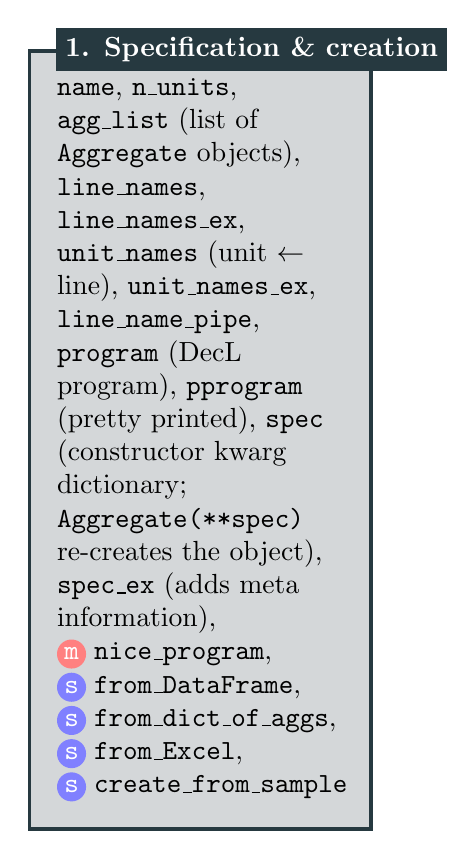
\begin{tikzpicture}
\node [mybox] (box){%
    \begin{minipage}{0.3\textwidth}\raggedright

\texttt{name},
\texttt{n\_units},
\texttt{agg\_list} (list of \texttt{Aggregate} objects),
\texttt{line\_names},
\texttt{line\_names\_ex},
\texttt{unit\_names} (unit $\leftarrow$ line),
\texttt{unit\_names\_ex},
\texttt{line\_name\_pipe},
\texttt{program} (DecL program),
\texttt{pprogram} (pretty printed),
\texttt{spec} (constructor kwarg dictionary; \texttt{Aggregate(**spec)} re-creates the object),
\texttt{spec\_ex} (adds meta information),
\texttt{\m nice\_program},
\texttt{\s from\_DataFrame},
\texttt{\s from\_dict\_of\_aggs},
\texttt{\s from\_Excel},
\texttt{\s create\_from\_sample}

    \end{minipage}
};
\node[fancytitle] at (box.north west) {1. Specification \& creation};
\end{tikzpicture}


%------------2. UPDATE ---------------
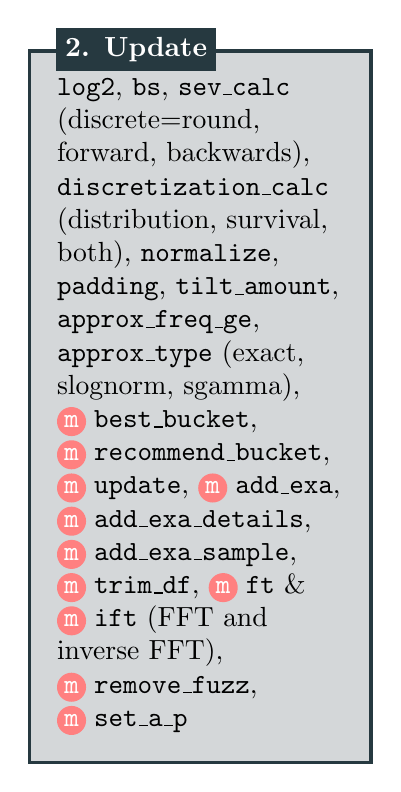
\begin{tikzpicture}
\node [mybox] (box){%
    \begin{minipage}{0.3\textwidth}\raggedright
    
\texttt{log2},
\texttt{bs},
\texttt{sev\_calc} (discrete=round, forward, backwards),
\texttt{discretization\_calc} (distribution, survival, both),
\texttt{normalize},
\texttt{padding},
\texttt{tilt\_amount},
\texttt{approx\_freq\_ge},
\texttt{approx\_type} (exact, slognorm, sgamma),
\texttt{\m best\_bucket},
\texttt{\m recommend\_bucket},
\texttt{\m update},
\texttt{\m add\_exa},
\texttt{\m add\_exa\_details},
\texttt{\m add\_exa\_sample},
\texttt{\m trim\_df},
\texttt{\m ft} \&
\texttt{\m ift} (FFT and inverse FFT),
\texttt{\m remove\_fuzz},
\texttt{\m set\_a\_p}

    \end{minipage}
};
\node[fancytitle] at (box.north west) {2. Update};
\end{tikzpicture}


%------------ 3. MOMENTS ---------------
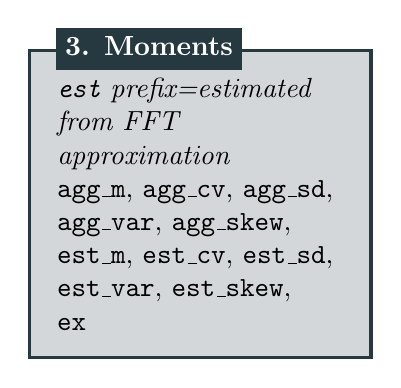
\begin{tikzpicture}
\node [mybox] (box){%
    \begin{minipage}{0.3\textwidth}\raggedright

{\it \texttt{est} prefix=estimated from FFT approximation} \\
\texttt{agg\_m},
\texttt{agg\_cv},
\texttt{agg\_sd},
\texttt{agg\_var},
\texttt{agg\_skew}, \\
\texttt{est\_m},
\texttt{est\_cv},
\texttt{est\_sd},
\texttt{est\_var},
\texttt{est\_skew}, \\
\texttt{ex}


    \end{minipage}
};
\node[fancytitle] at (box.north west) {3. Moments\vphantom{p}};
\end{tikzpicture}


%------------ 4. STATISTICAL FUNCTIONS ---------------
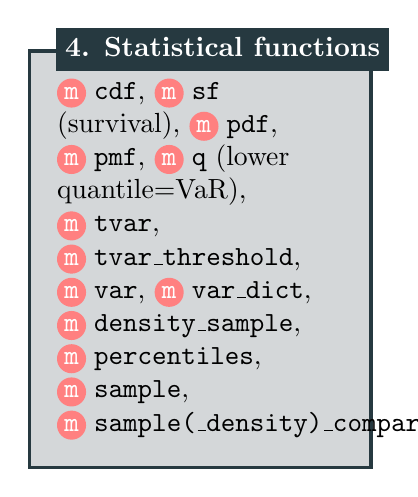
\begin{tikzpicture}
\node [mybox] (box){%
    \begin{minipage}{0.3\textwidth}\raggedright

\texttt{\m cdf},
\texttt{\m sf} (survival),
\texttt{\m pdf},
\texttt{\m pmf},
\texttt{\m q} (lower quantile=VaR),
\texttt{\m tvar},
\texttt{\m tvar\_threshold},
\texttt{\m var},
\texttt{\m var\_dict},
\texttt{\m density\_sample},
\texttt{\m percentiles},
\texttt{\m sample},
\texttt{\m sample(\_density)\_compare},

    \end{minipage}
};
\node[fancytitle] at (box.north west) {4. Statistical functions\vphantom{p}};
\end{tikzpicture}


\columnbreak


%------------ 5. VALIDATION ---------------
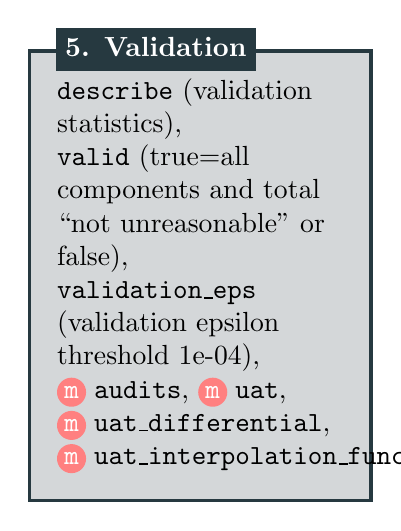
\begin{tikzpicture}
\node [mybox] (box){%
    \begin{minipage}{0.3\textwidth}\raggedright

\texttt{describe} (validation statistics),    \\
\texttt{valid}  (true=all components and total ``not unreasonable'' or false), \\
\texttt{validation\_eps} (validation epsilon threshold 1e-04),
\texttt{\m audits},
\texttt{\m uat},
\texttt{\m uat\_differential},
\texttt{\m uat\_interpolation\_functions}

    \end{minipage}
};
\node[fancytitle] at (box.north west) {5. Validation\vphantom{p}};
\end{tikzpicture}


%------------ 6. OUTPUT ---------------
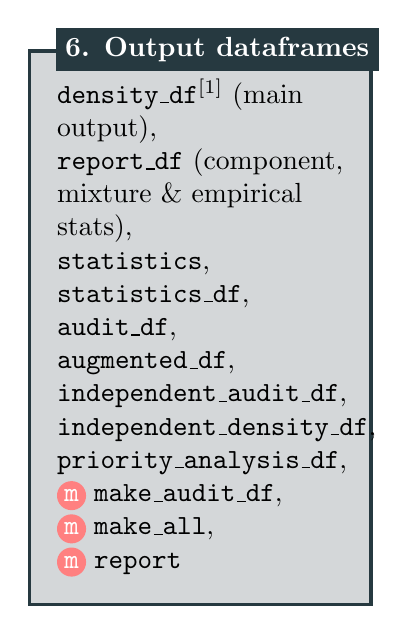
\begin{tikzpicture}
\node [mybox] (box){%
    \begin{minipage}{0.3\textwidth}\raggedright

\texttt{density\_df}${}^{[1]}$ (main output), \\
\texttt{report\_df}  (component, mixture \& empirical stats), \\
\texttt{statistics},
\texttt{statistics\_df},
\texttt{audit\_df},
\texttt{augmented\_df},
\texttt{independent\_audit\_df},
\texttt{independent\_density\_df},
\texttt{priority\_analysis\_df},
\texttt{\m make\_audit\_df},
\texttt{\m make\_all},
\texttt{\m report}


    \end{minipage}
};
\node[fancytitle] at (box.north west) {6. Output dataframes};
\end{tikzpicture}


%------------ 7. REINSURANCE ---------------
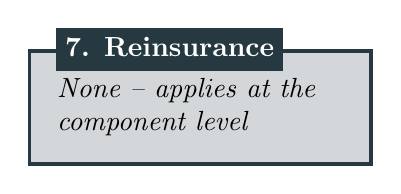
\begin{tikzpicture}
\node [mybox] (box){%
    \begin{minipage}{0.3\textwidth}\raggedright

{\it None -- applies at the component level}

    \end{minipage}
};
\node[fancytitle] at (box.north west) {7. Reinsurance\vphantom{p}};
\end{tikzpicture}



%------------ 8. VISUALIZTION ---------------
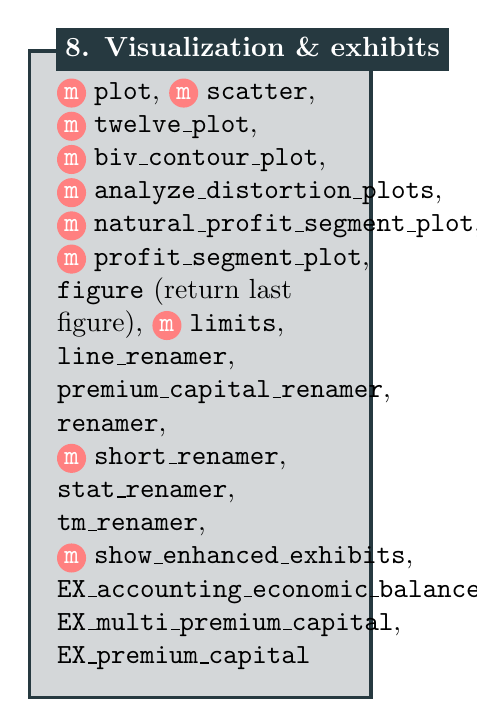
\begin{tikzpicture}
\node [mybox] (box){%
    \begin{minipage}{0.3\textwidth}\raggedright

\texttt{\m plot},
\texttt{\m scatter},
\texttt{\m twelve\_plot},
\texttt{\m biv\_contour\_plot},
\texttt{\m analyze\_distortion\_plots},
\texttt{\m natural\_profit\_segment\_plot},
\texttt{\m profit\_segment\_plot},
\texttt{figure} (return last figure),
\texttt{\m limits},
\texttt{line\_renamer},
\texttt{premium\_capital\_renamer},
\texttt{renamer},
\texttt{\m short\_renamer},
\texttt{stat\_renamer},
\texttt{tm\_renamer},
\texttt{\m show\_enhanced\_exhibits},
\texttt{EX\_accounting\_economic\_balance\_sheet},
\texttt{EX\_multi\_premium\_capital},
\texttt{EX\_premium\_capital}


    \end{minipage}
};
\node[fancytitle] at (box.north west) {8. Visualization \& exhibits\vphantom{p}};
\end{tikzpicture}

\columnbreak


%------------ 9. RISK ---------------
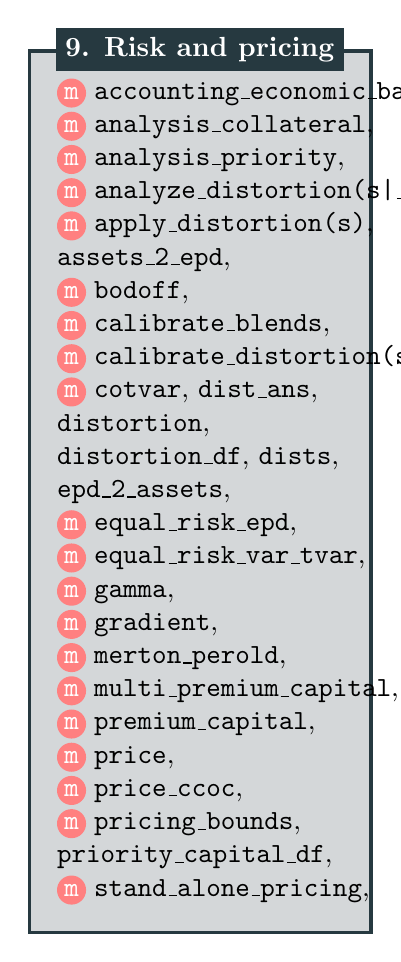
\begin{tikzpicture}
\node [mybox] (box){%
    \begin{minipage}{0.3\textwidth}\raggedright

\texttt{\m accounting\_economic\_balance\_sheet},
\texttt{\m analysis\_collateral},
\texttt{\m analysis\_priority},
\texttt{\m analyze\_distortion(s|\_add\_comps)},
%\texttt{\m analyze\_distortion\_add\_comps},
%\texttt{\m analyze\_distortions},
\texttt{\m apply\_distortion(s)},
%\texttt{\m apply\_distortions},
\texttt{assets\_2\_epd},
\texttt{\m bodoff},
\texttt{\m calibrate\_blends},
\texttt{\m calibrate\_distortion(s)},
%\texttt{\m calibrate\_distortions},
\texttt{\m cotvar},
\texttt{dist\_ans},
\texttt{distortion},
\texttt{distortion\_df},
\texttt{dists},
\texttt{epd\_2\_assets},
\texttt{\m equal\_risk\_epd},
\texttt{\m equal\_risk\_var\_tvar},
\texttt{\m gamma},
\texttt{\m gradient},
\texttt{\m merton\_perold},
\texttt{\m multi\_premium\_capital},
\texttt{\m premium\_capital},
\texttt{\m price},
\texttt{\m price\_ccoc},
\texttt{\m pricing\_bounds},
\texttt{priority\_capital\_df},
\texttt{\m stand\_alone\_pricing},
%\texttt{\m stand\_alone\_pricing\_work}


    \end{minipage}
};
\node[fancytitle] at (box.north west) {9. Risk and pricing};
\end{tikzpicture}


%------------  10. APPROXIMATIONS ---------------
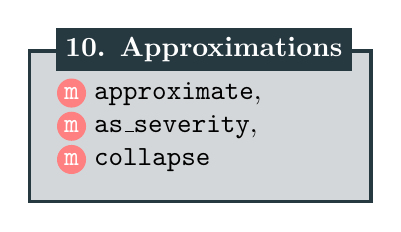
\begin{tikzpicture}
\node [mybox] (box){%
    \begin{minipage}{0.3\textwidth}\raggedright

\texttt{\m approximate},
\texttt{\m as\_severity},
\texttt{\m collapse}

    \end{minipage}
};
\node[fancytitle] at (box.north west) {10. Approximations};
\end{tikzpicture}


%------------ 11. META ---------------
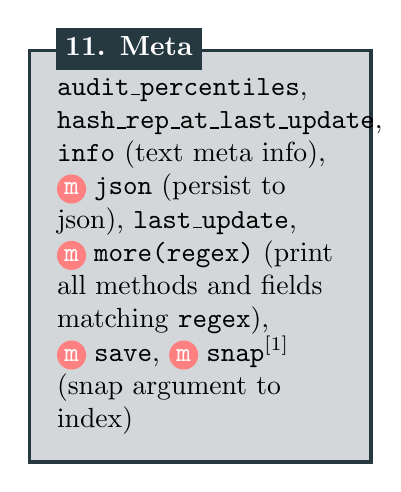
\begin{tikzpicture}
\node [mybox] (box){%
    \begin{minipage}{0.3\textwidth}\raggedright

\texttt{audit\_percentiles},
\texttt{hash\_rep\_at\_last\_update},
\texttt{info}  (text meta info),
\texttt{\m json} (persist to json),
\texttt{last\_update},
\texttt{\m more(regex)} (print all methods and fields matching \texttt{regex}),
\texttt{\m save},
\texttt{\m snap}${}^{[1]}$ (snap argument to index)

    
    \end{minipage}
};
\node[fancytitle] at (box.north west) {11. Meta\vphantom{p}};
\end{tikzpicture}

\bigskip \raggedright
{\bf Notes:} 

[1]: matches \texttt{Aggregate}

Any vectorizable input accepts numeric or iterable datatypes.  

Abbreviations: gcn=gross (subject), ceded, and net; stats: m=mean, cv=coefficient of variation, sd=standard deviation, var=variance, skew(ness); VaR=value-at-risk


% FOOTER
\makefooter

\end{multicols*}

\end{document}
